\documentclass[a4paper, openany]{memoir}

\usepackage[utf8]{inputenc}
\usepackage[T1]{fontenc} 
\usepackage[english]{babel}
\usepackage{amsmath}
\usepackage{amssymb}

\usepackage{booktabs}
\usepackage{fancyhdr}
\usepackage{float}
\usepackage{indentfirst}
\usepackage{graphicx}
\usepackage[linewidth=1pt]{mdframed}
\usepackage{multicol}
\usepackage{fancyvrb}

\pagestyle{fancy}
\fancyhf{}
\fancyhead[LE]{\leftmark}
\fancyhead[RO]{\rightmark}
\fancyhead[RE, LO]{PSD}
\fancyfoot[LE, RO]{\thepage}
\fancyfoot[RE, LO]{Pete Gautam}

\renewcommand{\headrulewidth}{1.5pt}

\chapterstyle{thatcher}
\setcounter{chapter}{5}

\begin{document}

\chapter{Software Process Improvement}
Software process improvement practices provide a structured way for a team to reflect on their process and identify opportunities for improvement. Below are some process improvement frameworks:
\begin{itemize}
    \item ISO 9001,
    \item Six Sigma,
    \item Capability Maturity Model (CMM).
\end{itemize}
A common feature of each of these frameworks is that they predefined the characteristics of a functioning software process. They do not allow for empirical measurement, goal setup and adjustments, which are more common in agile. So, these approaches are to software process improvement what the waterfall method is to software process itself. In particular, they predefined a particular feature of a mature quality in the software process.

However, CMM identifies the most mature software processes as optimising and describes it like Schwaeber describes empirical process control in the Scrum method. That is, they anticipate that software project transitions through less mature structures (which are defined) before reaching the most mature (which is optimising). The less mature states include:
\begin{itemize}
    \item repeatable software processes, which is where a team knows how to repeatedly apply predefined set of activities to software development.
    \item defined software process is documented, which is when the team has a resource that they can refer to in order to apply the software process.
    \item managed software process, which is where the team is actively managing the software process and applying the controls as appropriate.
    \item optimising software process, which is the most mature form.
\end{itemize}

\section{Principals for agile process improvement}
Any measurement/data gathered in one project cannot be transferred to another project; they are domain-specific. This is because they are only relevant to the particular activities taken place within the empirically measured software project being improved.

Moreover, improvement is an ongoing activity. The software project is iteratively developed through a series of sprints. In a similar way, the software process must also improve iteratively as the nature of the software project changes and more opportunities for improvement are discovered.

Also, the process requires the whole team to participate in the process improvement activity. There are 2 reasons for this:
\begin{itemize}
    \item It maximises the data gathered and the ideas generated for improving the software process.
    \item By involving everyone, it creates buy-in for the actions proposed. The whole team is asked to take part and make decisions about the process, so they feel like they have some stake in the decision.
\end{itemize}

During the process, we have the best effort assumption. That is, everyone is trying their hardest to ensure the sprint was successful. This implies that
\begin{itemize}
    \item working harder won't improve the process. They are already working as hard as possible.
    \item blaming is pointless. Every member is working the hardest, so it won't remedy the failures by working harder. It is also counterproductive. A culture of blaming creates tension within the team and prevents effective remedies being identified.
\end{itemize}

Also, we would like to identify the root cause and remedy it during the process improvement activity, not surface-level symptoms. We are looking for the real reasons why a software process has failed.

\section{Process improvement process}
The following is the process improvement process cycle.
\begin{figure}[H]
    \centering
    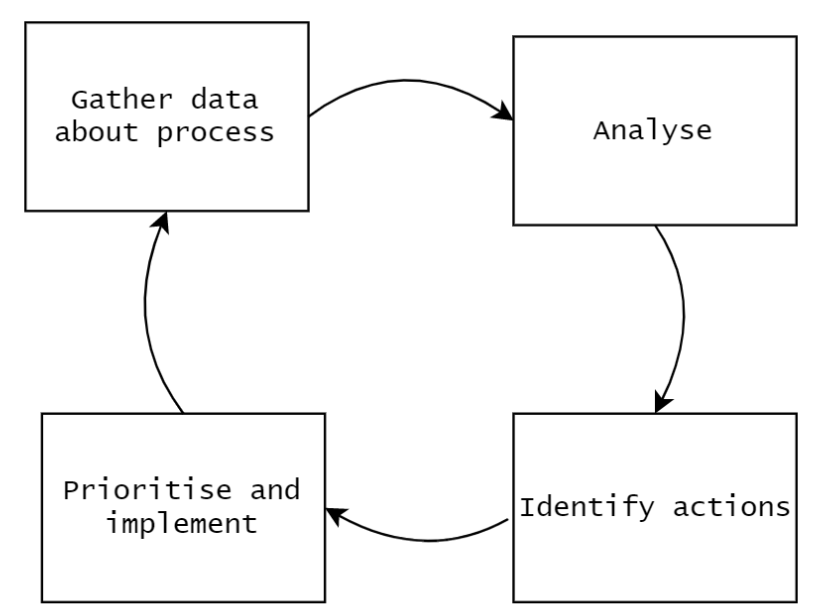
\includegraphics[scale=0.4]{src/6 process improvement process.PNG}
    \caption{Process improvement process}
\end{figure}
\noindent As we can see, there are 4 parts to it:
\begin{itemize}
    \item We gather data about the process from team members and alternate tools (e.g. the version control tool, issue tracker and static analysis).
    \item We analyse and synthesise data to find the root cause of the issue.
    \item We identify actions to address the root cause identified.
    \item We prioritise and implement after choosing which ones to implement within the next sprint.
\end{itemize}
This process is iterative and ongoing. In particular, previously implemented priorities feed back into data gathering process at the end of the next sprint.

\subsection{Retrospectives}
In the Scrum method, the process improvement process is realised by a retrospective meeting. This occurs at the end of the sprint, after the review meeting with the customer. Typically, the whole team participates and the Scrum master acts as a facilitator, particularly in new teams. Some teams also include the product owner and the customer, but this can make data gathering harder- the team might not be comfortable explaining their experience in front of the customer. 

The retrospective meeting should last at least 30 minutes to allow for proper data gathering. It will be longer for longer sprints, since more issues should have arisen over the longer time period. Nonetheless, it should not last more than half a day. It should not consume too much of the project time.

There are two types of data sources for the retrospective meeting:
\begin{itemize}
    \item The project artifacts, which can be used to gather objective evidence about problems. However, it needs to be interpreted carefully.
    \item The team members, who can provide very detailed insight and reflections on the encountered problems, and help to identify the subsequent actions. However, this data is subjective and might need to be validated with objective evidence from project artifacts.
\end{itemize}
Typically, we make use of both sources of data. They complement each other.

We now consider the general method for the retrospective. The team first chooses a template board (e.g. a whiteboard divided into different themes). The team populates the board using sticky notes and places the notes on the right theme. The team then groups similar items, within and across the themes. The team votes on the primary issues for discussion, which reveals the root cause of the issue. Finally, the team chooses actions for improvement.

There are many templates available for data gathering, which have different themes. Some common templates are:
\begin{itemize}
    \item stop, start, continue.
    \item mad, sad, glad.
    \item loved, learned, lacked/longed for,
    \item sailboat.
\end{itemize}
The different templates fill in the issues in different ways. For example, in the stop, start, continue method, the three themes are:
\begin{itemize}
    \item stop- what did we do that did not help and we should stop?
    \item start- what should we begin doing that we aren't doing yet?
    \item continue- what did we do well and should keep doing?
\end{itemize}
The figure below shows a stop, start, more board that has been grouped within the themes.
\begin{figure}[H]
    \centering
    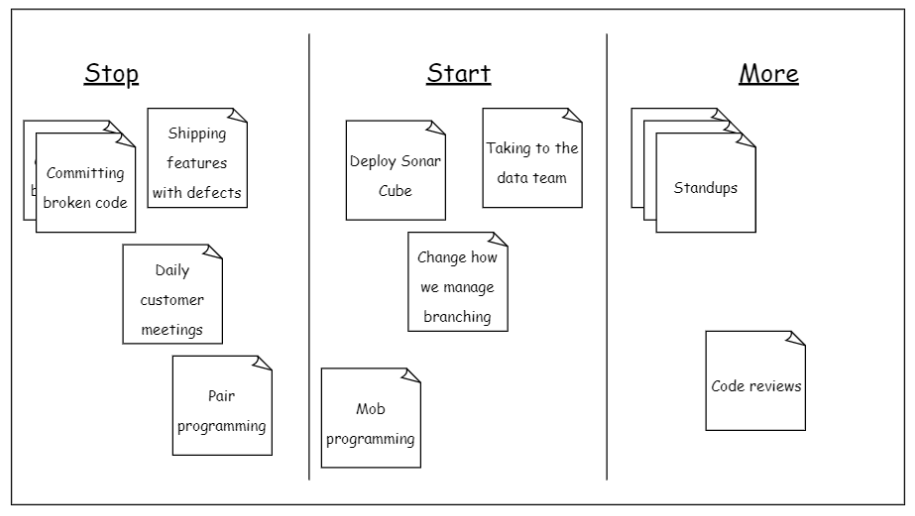
\includegraphics[scale=0.5]{src/6 stop start more.PNG}
    \caption{A stop, start, more board}
\end{figure}
\noindent The issues have been grouped together within themes, e.g. 2 members were concerned about committing broken code. However, they haven't been group across themes yet. For example, group programming and review are in stop (pair programming), start (mob programming) and more (code reviews). These should be discussed together.

The start section indicates candidate solutions proposed by the member instead of underlying solution. A root cause analysis shows why the member wants to adopt the recommendation, and can help find a better solution. Moreover, the team has not yet voted on issues for discussion. This does not necessarily correspond to the number of people who highlighted that issue.

The data on the template board are observations of the software process. They are not explanations of the reasons why those observations were made. Without knowing the underlying issue, we cannot identify an effective solution that can remedy that problem and stop it from occurring in the future. We can do a root cause analysis to remedy the real, underlying problem rather than the superficial observations.

One way of identifying the root cause is by using the 5 whys technique. Here, we ask why an observation was seen again and again until we identify a root cause. If we can identify the solution that will prevent the high-level cause from occurring, then the cause must be the root cause. In the 5 whys process, we do not necessarily ask the question why 5 times. On average, we need 5 whys to get to the root cause, however it might take a little more or a little less in a particular case.

After identifying the actions, we need to implement them. We need to monitor and measure the progress as part of the software process. We create tickets as appropriate for the next milestone/release. We ensure that every action has a team member assigned to it. We include previous decisions in future retrospectives to be re-evaluated. Furthermore, we also review the process review process.

\section{Continuous process improvement}
Retrospectives only take place at discrete periods of time (e.g. 2/4 weeks). This can be problematic. For instance, a problem might be identified early in the sprint, but doesn't get highlighted/fixed until the next retrospective/sprint. Moreover, as time goes on, it becomes harder to recall the issue- we might misremember or even forget it.

To remedy this, we can use continuous retrospective. So, rather than waiting until the end of the sprint, we conduct a mini-retrospective as soon as a problem is identified. This means that problems are dealt with quickly and effectively. However, not everyone might be able to make it to this meeting. So, the solution agreed to might not be something that everyone agrees to, and the best solution (or even the root cause) might not get identified. Also, continual change to the retrospective might disrupt software process in terms of productivity.

We can use a hybrid approach to avoid these issues. We diagnose and recommend a solution to a problem within the sprint, but this does not get implemented until it is discussed with everyone in the retrospective.

\section{Improving process improvement}
Retrospectives can become stale if we conduct them in the same way all the time. It is important to:
\begin{itemize}
    \item vary their structure by using a different template or including different participants.
    \item reflect on the retrospective itself at the end of the meeting to identify how we can improve the process.
    \item experiment with different frequencies. For instance, doing retrospectives again and again becomes less valued since the process is already quite optimised. It is a good idea to make them less frequent as time goes on.
    \item allow other team members to facilitate.
\end{itemize}

In summary, process improvement is an essential quality assurance process within software engineering. It has the potential to enhance the quality of all other software process practices.

\end{document}